\section{Overall Description}
\label{sec:overall_description}

\subsection{Product Perspective}
The product to be is a new open-source feed reader, with no predecessors, that will compete with existing solutions on the market by offering an low-overhead and minimalistic interface without the need of a web-based back-end. The goal is to give users a simple but powerful feed reading solution.

\subsection{Product Features}
\label{sec:product_features}
\begin{figure}[hbt]
\centering
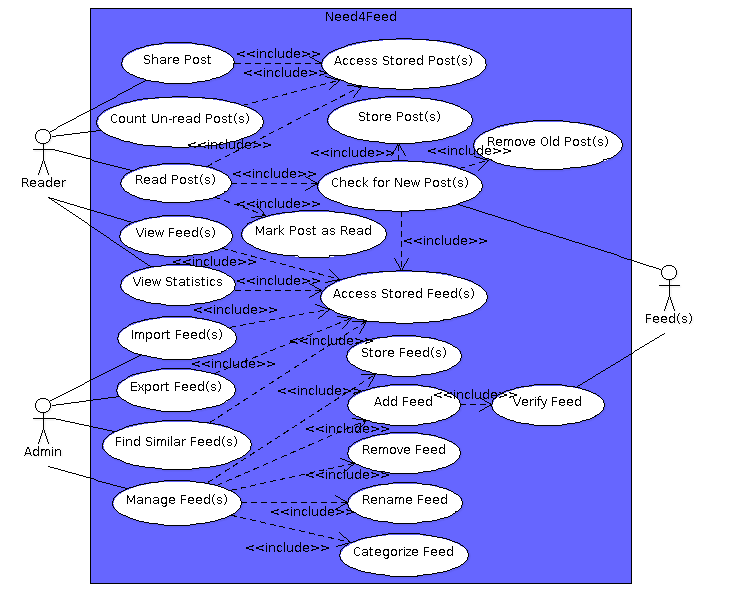
\includegraphics[width=\textwidth]{./images/UseCaseDiagramGeneralFull.png}
\caption{Complete use case of the major features}
\label{fig:use_case}
\end{figure}
The product's use case diagram is shown in figure~\ref{fig:use_case}, where actors, major features and included sub-features are displayed. The overall feature can be described as a feed library where the user can organize feeds as well as view posts. The actors of the product are Reader and Admin, which are subsets of User, as well as Feed(s). Feed(s) are not a person but still an actor to the product as it provides data.\\ \\
The major features of the product are:

\begin{itemize}
  \item Share Post
  \item Count Un-read Post(s)  
  \item Read Post(s)
  \item View Feed(s)
  \item Import Feed(s)
  \item Export Feed(s)
  \item Find Similar Feed(s)
  \item Manage Feed(s)
\end{itemize}
Underneath the major features are a set of sub-features to describe the flow of the product.\\ \\
The major user interfaces are:

\begin{itemize}
  \item View Categories
  \item View Feeds
  \item View Posts
  \item View Post
\end{itemize}
The product shall include these four user interfaces to enable the user to utilize all the major features of the product.


\subsection{Operating Environment}
The environment for the product shall be Android\cite{android}, which is an operating system for touchscreen mobile devices. The product shall be supported for Android version 2.2, \textit{Froyo}, up to 4.1, \textit{Ice Cream Sandwich}. The product shall comply the hardware requirements that are required by the specified Android versions. 


\subsection{User Documentation}
To complement the product a user manual shall be created. This manual shall contain common user scenarios as well as descriptions of all options available throughout the user interface. An optional addition would be a developer’s guide to encourage outsiders to get involved.

